In this section, I present my 
adaptivity analysis based on static program analysis as the second part of 
the full-spectrum adaptivity analysis as in Figure~\ref{fig:structure}. 
% \section{Introduction}
% \label{sec:static-intro}
% 
\paragraph{{Static analysis for adaptivity}}
% The high level architecture of our static analysis framework is presented in 
%  Figure~\ref{fig:structure}. The input of the analysis is a labeled program P for which the adaptivity A is defined by means of a trace-based definition, as discussed above. In order to estimate an upper bound on A, our program analysis first transforms the program P into static single assignment (SSA) form. The goal of this step is to guarantee that each variable is assigned only once. We show the result of this transformation applied to our two rounds strategy example in Figure~\ref{fig:dcfgraph_tworound}(a). 
%  This transformation, when applied to a loop, introduces some extra variables that serve as intermediate storage. For example, in~\ref{fig:dcfgraph_tworound}(a) there is a new instruction $[(i_3,i_1,i_2),(a_3,a_1,a_2)]$ after the loop. This instruction asserts that the value of the new variables $i_3$ and $a_3$, depending on the execution step, may come from $i_2$ or $i_2$, $a_1$ or $a_2$, respectively. The transformation of a program into SSA form preserves the execution traces, and so, in turns, it preserves the adaptivity. 
% Let us see now how o
Our static analysis provides an upper bound on the adaptivity for this example as follows.
% The high level architecture of our static analysis framework is presented in 
% \jl{Still stick on the two rounds strategy example, which has the aforementioned adaptivity $2$ according our definition, we now present our static analysis which is able to provide an upper bound on the adaptivity, taking the labeled program as input, see Figure~\ref{fig:overview-example}(b). }
% Based on the Ω The input of the analysis is a labeled program P for which the adaptivity $A(c)$ is defined in our formal model as discussed above. 
%  transforms the program P into static single assignment (SSA) form. The goal of this step is to guarantee that each variable is assigned only once. We show the result of this transformation applied to our two rounds strategy example in Figure~\ref{fig:dcfgraph_tworound}(a). 
%  This transformation, when applied to a loop, introduces some extra variables that serve as intermediate storage. For example, in~\ref{fig:dcfgraph_tworound}(a) there is a new instruction $[(i_3,i_1,i_2),(a_3,a_1,a_2)]$ after the loop. This instruction asserts that the value of the new variables $i_3$ and $a_3$, depending on the execution step, may come from $i_2$ or $i_2$, $a_1$ or $a_2$, respectively. The transformation of a program into SSA form preserves the execution traces, and so, in turns, it preserves the adaptivity. 
%  Our framework l ${\THESYSTEM}$
% \jl{Similar as the dependency graph in Figure~\ref{fig:overview-example}(c), {\THESYSTEM} constructs a "may" dependency graph between assigned variables whose dependency both considers control flow and data flow, with the help of some program analysis techniques. To be precise, 
% this algorithm analyzes the data flow relations through variables assigned in every command, based on an abstract control flow graph shown in Figure~\ref{fig:dcfgraph_tworound}(a).} 
% \jl{
 {\THESYSTEM} constructs a program-based dependency graph, for our example we show this graph in Figure~\ref{fig:overview-example}(c). The edges of this graph are built by considering both control flow and data flow between assigned variables (the algorithm is presented in Section~\ref{sec:alg_edgegen}). The weight of every vertex is estimated by using a reachability-bound estimation algorithm (presented in Section~\ref{sec:alg_weightgen}), which can be symbolic and provide a sound upper bound on the weight of the corresponding vertex in the execution-based dependency graph. For instance, the weight $k$ of the vertex $x^{3}$ in Figure~\ref{fig:overview-example}(c) is a sound upper bound on the weight $w_k$ of vertex $x^{3}$ in Figure~\ref{fig:overview-example}(b), with the same starting trace. The soundness of this step is proved in Theorem~\ref{thm:addweight_soundness}.
% Then {\THESYSTEM} computes the adaptivity upper bound through this program-based dependency graph, 
% to approximate the adaptivity defined in the formal model above over the Figure~\ref{fig:overview-example}(b).
% }
%
% through variables assigned in every command, based on an abstract control flow graph shown in Figure~\ref{fig:dcfgraph_tworound}(a).
% \jl{Todo:Add some interesting points of this abstract graph of two round here. Do we want to keep the abstract-cfg here? which is a part of the analysis technique, I think maybe just the final weighted dcfg is enough}
% (1)
%  In this abstract control flow graph, every vertex is a label,
%  corresponding to a label command in the program.
% Each directed 
%  edge represents an abstract transition 
%  between two control locations, i.e., the labels of two commands (we call the labels also control location and they refer to the same thing), 
%  where the second labeled command will be executed after execution of the command with first label.
%  The abstract transition contains a set of difference constraints for variables, generated by abstracting the command of the first labeled.} \wq{The data control dependency graph generated by our algorithm for our two round strategy example is presented in Figure~\ref{fig:dcfgraph_tworound}(b). We can easily see in the graph, that the node $x^{3}$ from the query assignment at line $3$ may depend on the node $j^{1}$ from control flow and node $a^{5}$ may depend on $x^{3}$ from data flow.
%
%  \jl{ Please pay attention to the graph in Figure~\ref{fig:dcfgraph_tworound}(b), every node also has a weight. As a reminder, we also have weight for every node in the dependency graph from our trace semantics in Figure~\ref{fig:overview-example}(c), which stands for the maximal number of times the node (also the statement) appears in the possible traces. In our static analysis, we provide a sound upper bound on this weight from the trace(execution) by performing reachability bound analysis on every statement. The reachability bound is a upper bound on the number of the target command may be reached in a program, which is used as the weight of nodes in our static analysis based data control depdendency graph. The weight can be symbolic, as indicated by the weight $k$ of node $x^{3}$ in Figure~\ref{fig:dcfgraph_tworound}(b).}
 %
% {To be precise, in order to construct the program-based dependency graph,
% $\THESYSTEM$ approximates the vertices and annotations in the first step.
% Then it
% analyzes the data flow relations for approximating the edges between every vertex,
% as well as the quantitative information for approximating the weights of each vertex.}
%  on the dependency depth. Then, it derives a weighted data dependency graph as in Figure~\ref{fig:dcfgraph_tworound}(b), aiming to approximate the graph modeled from execution traces in Figure~\ref{fig:overview-example}(c).
%  Starting from the Figure~\ref{fig:dcfgraph_tworound}(a), $\THESYSTEM$ first generate an abstract control flow graph.
%   In this abstract control flow graph, every vertex is a label,
%  corresponding to a label command in the program.
% Each directed 
%  edge represents an abstract transition 
%  between two control locations, i.e., the labels of two commands (we call the labels also control location and they refer to the same thing), 
%  where the second labeled command will be executed after execution of the command with first label.
%  The abstract transition contains a set of difference constraints for variables, generated by abstracting the command of the first labeled.
%  through this graph and constraint for every transition, 
%
% and compute the transition closure for every abstract transition.
% By solving the closure with the invariants of variables involved in this closure for every transition, 
% we compute the symbolic reachability bound of every commands corresponding to 
% this transition.
 %
 %  (3)
%  in the meantime, this algorithm perform a feasible data-flow analysis through the reachable definition algorithm. 
%  By generating set of all the reachable variables at location of label $l$ in the program $c$.
% For every labelled variable $x^l$ in this set, 
% the value assigned to that variable
% in the assignment command associated to that label is reachable at the entry point of  executing the command of label $l$.
% (4)Then,  by removing the edges between locations where the variables associated to that labeled command isn't reachable from the second location,
% we refined this graph into a weighted-data dependency graph.
 
% $\THESYSTEM$ first performs a simple pass on program collecting the identical vertices
%  and query annotations as in Figure~\ref{fig:overview-example}(c).
% Then, $\THESYSTEM$ performs a feasible data-flow analysis through the reachable definition algorithm, 
% % and refined this graph
% % into the weighted data dependency graph as in Figure~\ref{fig:dcfgraph_tworound}(b), 
% as the approximation of edges in Figure~\ref{fig:overview-example}(b).
%  As a reminder, we also have weight for every node in the dependency graph from our trace semantics as in Figure~\ref{fig:overview-example}(b), which stands for the maximal number of times the node (also the statement) appears over all the possible traces. 
% Similarly,  $\THESYSTEM$ also 
% % infers a symbolic 
% computes a reachability bound as the approximated maximal number of visiting times for each vertex in the program-based dependency graph,
% % by reachability bound for every
% % labeled variable.
% % In our static analysis, we provide a sound upper bound on this weight from the trace(execution) 
% by performing a reachability bound analysis. 
% This reachability bound is a upper bound on the number of the target command may be reached in a program, which is used as the weight of nodes in the program-based dependency graph generated from static analysis.
% % based data control dependency graph. 
% The weight is symbolic, as indicated by the weight $k$ of node $x^{3}$ in Figure~\ref{fig:overview-example}(c).
% Then
% $\THESYSTEM$ generates the program-based dependency graph as in Figure~\ref{fig:overview-example}(c), as a
% % an approximated graph as in 
% approximation for the graph in 
% %  In Figure~\ref{fig:dcfgraph_tworound}(b), every node also has a weight. 
% Figure~\ref{fig:overview-example}(b).}
%  Figure~\ref{fig:dcfgraph_tworound}(b).
%   The upper bound of reaching times of each variable, which performs as the weight of node in the .  estimated by  reachablility it refines this control flow graph into a weighted data-dependency graph, through the data flow and reaching bound analysis results. as well as the reaching times of each variable 
% \wq{The last step of {\THESYSTEM} is that} it finds the longest walk in the weighted data control flow graph w.r.t. the query variables,
% and return the number of query vertices it traversed alongside.
% To be more specific,
% (1)
%  In this abstract control flow graph, every vertex is a label,
%  corresponding to a label command in the program.
% Each directed 
%  edge represents an abstract transition 
%  between two control locations, i.e., the labels of two commands (we call the labels also control location and they refer to the same thing), 
%  where the second labeled command will be executed after execution of the command with first label.
%  The abstract transition contains a set of difference constraints for variables, generated by abstracting the command of the first labeled.
%  (2) Then through this graph and constraint for every transition, we infer the  invariant for every variable,
% and compute the transition closure for every abstract transition.
% By solving the closure with the invariants of variables involved in this closure for every transition, 
% we compute the symbolic reachability bound of every commands corresponding to 
% this transition.
%  (3)
%  in the meantime, this algorithm perform a feasible data-flow analysis through the reachable definition algorithm. 
%  By generating set of all the reachable variables at location of label $l$ in the program $c$.
% For every labelled variable $x^l$ in this set, 
% the value assigned to that variable
% in the assignment command associated to that label is reachable at the entry point of  executing the command of label $l$.
% (4)Then,  by removing the edges between locations where the variables associated to that labeled command isn't reachable from the second location,
% we refined this graph into a weighted-data dependency graph.
%  In the last step, 
 $\THESYSTEM$ search a walk on this graph which overapproximate the adaptivity of the program (this is done by an algorithm
 $\pathsearch$ presented in  Section~\ref{sec:alg_adaptcompute}). 
%  finds a finite walk on this graph.
% This finite walk traverses the maximum times of query variables, 
% and the visiting time of every vertex on this walk is restricted by its weight.
% The maximum number of vertices visited on this walk which correspond to query variables, is the final estimated adaptivity upper bound, for the program.
For instance, in Figure~\ref{fig:overview-example}(c), $\pathsearch$ first finds a path $l^6:{}^1_1 \to a^5: {}^k_1 \to x^3: {}^k_1$, and then approximate a walk with this path.
Every vertex on this walk is visited once, and the number of vertices with query annotation $1$ traversed in this path is $2$, which is the upper bound we expect.
It is worth to note here that even though the node $x^3$ has weight depending on $k$, 
it is only visited once, similarly for $l^6$, hence the overall upper bound on the adaptivity is 2, as we expect.
% By defining it as the finite walk, and restricting the visiting time of each node to its weight, 
% it gives us significant improvement on the accuracy in terms of program cost analysis, comparing with computing the longest weighted path in the state-of-art graph-based program cost analysis works.
%  For analyzing the visiting times of each variable, we 
% \wq{Finally, we reach our analysis algorithm ${\THESYSTEM}$. To bound the longest path is Figure~\ref{fig:simpl-two-round-graph}(c), we decide to build a graph as well. To this end, {\THESYSTEM} constructs a variable-based weighted directed dependency graph where nodes are annotated variables and edges showing the may-dependency of variables. The may-dependency here considers both the data dependency and control dependency and the variables assigned with a query answer has weight $1$ and other variables have no weight. Hence, the estimated upper bound of adaptivity is the weight of most weighted path in the graph.  In Figure~\ref{fig:dcfgraph_tworound}(b), the most weighted path is the dashed one, with weighted node in dashed circle and normal node in standard circle. The weight of that path is $2$. In this example, {\THESYSTEM} produces an upper bound $2$, to the adaptivity $2$ we obtained before, showing its power of a tight estimation. 
% }
%  
% \begin{figure} 
% \centering
%   \begin{subfigure}{.45\textwidth}
%   \begin{centering}
% %   \todo{abstract-cfg for two round}
% \begin{tikzpicture}[scale=\textwidth/18cm,samples=200]
% \draw[] (-5, 10) circle (0pt) node{{ $0$}};
% \draw[] (0, 10) circle (0pt) node{{ $1$}};
% \draw[] (0, 7) circle (0pt) node{\textbf{$2$}};
% \draw[] (0, 4) circle (0pt) node{{ $3$}};
% \draw[] (0, 1) circle (0pt) node{{ $4$}};
% \draw[] (-5, 1) circle (0pt) node{{ $5$}};
% % Counter Variables
% \draw[] (3, 7) circle (0pt) node {\textbf{$6$}};
% \draw[] (3, 4) circle (0pt) node {{ $ex$}};
% %
% % Control Flow Edges:
% \draw[ thick, -latex] (-4.5, 10)  -- node [above] {$a \leq 0$}(-0.5, 10);
% \draw[ thick, -latex] (0, 9.5)  -- node [left] {$j \leq k$} (0, 7.5) ;
% \draw[ thick, -latex] (0, 6.5)  -- node [left] {$\top$}  (0, 4.5);
% \draw[ thick, -latex] (0, 3.5)  -- node [right] {$x \leq \max(\dbdom)$} (0, 1.5) ;
% \draw[ thick, -latex] (0, 1)  -- node [above] {$j \leq j - 1$} (-4.5, 1) ;
% \draw[ thick, -latex] (-5, 1.5)  -- node [left] {$a \leq a + x$} (-0.5, 7)  ;
% \draw[ thick, -latex] (0.5, 7)  -- node [above] {$\top$}  (2.5, 7);
% \draw[ thick, -latex] (3, 6.5)  -- node [left] {$\top$} (3, 4.5) ;
% \end{tikzpicture}
%  \caption{}
%   \end{centering}
%   \end{subfigure}
%   \begin{subfigure}{.5\textwidth}
%   \begin{centering}
%   \begin{tikzpicture}[scale=\textwidth/18cm,samples=200]
% \draw[] (0, 10) circle (0pt) node
% {{ $a^0: {}^1_{0}$}};
% \draw[] (0, 7) circle (0pt) node
% {\textbf{$x^3: {}^{k}_{1}$}};
% \draw[] (0, 4) circle (0pt) node
% {{ $a^5: {}^{k}_{0}$}};
% \draw[] (0, 1) circle (0pt) node
% {{ $l^6: {}^{1}_{1}$}};
% % Counter Variables
% \draw[] (5, 9) circle (0pt) node {\textbf{$j^2: {}^{1}_{0}$}};
% \draw[] (5, 6) circle (0pt) node {{ $j^4: {}^{k}_{0}$}};
% %
% % Value Dependency Edges:
% \draw[ ultra thick, -latex, densely dotted,] (0, 1.5)  -- (0, 3.5) ;
% \draw[ ultra thick, -latex, densely dotted,] (0, 4.5)  -- (0, 6.5) ;
% \draw[ thick, -latex] (0, 7.5)  -- (0, 9.5) ;
% \draw[ thick, -Straight Barb] (1.5, 3.5) arc (120:-200:1);
% \draw[ thick, -Straight Barb] (6.5, 6.5) arc (150:-150:1);
% \draw[ thick, -latex] (5, 6.5)  -- (5, 8.5) ;
% % Control Dependency
% \draw[ thick,-latex] (1.5, 7)  -- (4, 9) ;
% \draw[ thick,-latex] (1.5, 4)  -- (4, 9) ;
% \draw[ thick,-latex] (1.5, 7)  -- (4, 6) ;
% \draw[ thick,-latex] (1.5, 4)  -- (4, 6) ;
% \end{tikzpicture}
% \caption{}
%   \end{centering}
%   \end{subfigure}
%     \vspace{-0.3cm}
%     \caption{(a) Example of data-flow analysis results for two rounds of adaptivity (b) The  weighted data-dependency graph from static analysis result.}
%     \vspace{-0.5cm}
%     \label{fig:dcfgraph_tworound}
% \end{figure}
%
\paragraph*{Related Work} 
Our algorithm in Section~\ref{sec:algorithm} is influenced by many areas of static program analysis such as effect systems, control-flow analysis, and data-flow analysis~\cite{ryder1988incremental}. The idea of statically estimating a sound upper bound for the adaptivity from the semantics is indirectly inspired from prior work on cost analysis via effect systems~\cite{cciccek2017relational,radivcek2017monadic,qu2019relational}. The idea of defining adaptivity using data flow is inspired by the work of graded 
Hoare logic~\cite{gaboardi2021graded}, which reasons about data flows as a resource. 
%
One of the most important ingredients of our work is the estimation of the program-based dependency graph. 
There are many ways to construct a dependency graph statically.
Some of the most related work focuses on the testing of graphical user interfaces (GUIs), using an event graph. For example, \cite{memon2007event} proposes an event-flow model using an algorithm to construct an event-flow graph, representing all the possible event interactions. This event-flow graph has a vertex for every GUI event such as click-to-paste and an edge between pairs of events that can be performed immediately one after the other. Our program-based dependency graph uses the edge to track the may-dependence of one variable with respect to another variable. The main difference is in the way the graph is constructed. {\THESYSTEM} relies on the structure of the target program, while the event-flow model only considers the event type. Another work \cite{arlt2012lightweight} constructs a weighted event-dependency graph, capturing data dependencies between events by analyzing bytecode. Every weighted edge indicates a dependency between two events, meaning one event possibly reads data written by the other event, with the weight showing the intensity of the dependency (the quantity of data involved). Our approach of generating the program-based dependency graph shares the idea of tracking data dependency via static analysis on the source code. However, because of the different domains, we care about assigned variables, and we use the weight in a different way to find a finite walk in the graph.
% WCET on systems: \cite{} 
% [GustafssonEL05]Towards a Flow Analysis for Embedded System C Programs
% --> abstract interpretation.
% --> on embedded system of c program
% [AlbertAGP08] Automatic Inference of Upper Bounds for Recurrence Relations in Cost Analysis
% --> invariant generation through ranking functions
%
% General While langue:
% [BrockschmidtEFFG16]
% Analyzing Runtime and Size Complexity of Integer Programs
% --> invariant generation through ranking functions
% [AliasDFG10] Multi-dimensional Rankings, Program Termination, and Complexity Bounds of Flowchart Programs
% --> invariant generation through ranking functions
% [Flores-MontoyaH14]Resource Analysis of Complex Programs with Cost Equations
% --> invariant generation through cost equations or ranking functions
%
% [GulwaniJK09]Control-flow Refinement and Progress Invariants for Bound Analysis
% --> program abstraction and invariant inference
% []Bound Analysis using Backward Symbolic Execution
% --> program abstraction and invariant inference
%
% [CicekBG0H17]relational Cost Analysis 0
% Monadic refinements for relational cost analysis
% [RajaniG0021]A unifying type-theory for higher-order (amortized) cost analysis
% --> type-system
Moreover, the state-of-art data-flow analysis techniques do not
consider the quantitative information on how many times each variable is dependent on the other. Our weight estimation is inspired by
% (specifically in the case if
% the data-flow is nested in iterations of recursion into consideration). 
 works in program complexity analysis and worst case execution time analysis areas, focusing on analyzing the cost of the entire program. 
The techniques are based on
type system~\cite{CicekBG0H17, RajaniG0021}, Hoare logic~\cite{CarbonneauxHS15}, abstract interpretation~\cite{GustafssonEL05, HumenbergerJK18},
invariant generation through cost equations or ranking functions~\cite{BrockschmidtEFFG16,AlbertAGP08,AliasDFG10,Flores-MontoyaH14}
or a combination of program abstraction and invariant inferring~\cite{GulwaniZ10, SinnZV17,GulwaniJK09}.
In general, these techniques give the approximated upper bound of the program's total running time or resource cost.
However, they failed to consider the case where the cost -- the adaptivity-- could decrease when there isn't a dependency relation between variables.


% \section{Static Program Adaptivity Analysis -- $\THESYSTEM$}
% \label{sec:static-adapfun}
% 
% I discuss the vertices and edge of the
% abstract control flow graph for a program $c$, $\absG(c)$.
% In the abstract control flow graph,
% every 
% vertex corresponds to the unique
% label.
The abstract control flow graph is a control flow graph, with annotations on every edge. It is constructed as follows.
\paragraph*{Vertices of Abstract Control Flow Graph}
The abstract control flow graph enriches the standard control flow graph vertices set with
one extra label, $l_{lex}$ for each program $c$.
Specifically,
the vertices of this graph is the set of $c$'s labels with an exit label $l_{ex}$, 
\[ 
  \absV(c) = labels(c)\cup\{l_{ex}\}
\]
%  corresponding to a label command in the program.

Overall, the vertices can be easily collected and the key point of construction of the abstract execution control flow graph for a program is the abstract execution trace, 
which relies on the abstraction of expression and abstract transition (we also call it abstract event), I will discuss in the following section.

\paragraph*{Edges of Abstract Control Flow Graph}
  The edge in the abstract control flow graph comes from the abstract execution trace of the program. 
  The abstract execution trace, an abstract representation of the execution, consists of a list of abstract transitions. 
  Then, every abstract transition in the abstraction execution trace corresponds to an edge in the abstract control flow graph.
  In another word, the edge $(l_1, dc, l_2)$ in the abstract control flow graph, represents an abstract transition 
 from $l_1$ to $l_2$, with a set of difference constraints $dc$. 
 Also notice, the difference constraints generated during the abstract transition appears in the edge as annotation.
% \wq{
  %  To make it easy to understand, 
  % }  
%
\paragraph{Edge Construction Step 1: Expression Abstraction}

The expression assigned to the variable on the left hand of the assignment command is abstracted to an abstract value: (adopted from the expression abstraction method in paper \cite{sinn2017complexity}). The abstract value is expressed in the form of Difference constraint, denotated as $DC : \mathcal{VAR} \cup \constdom \to \mathcal{\mathcal{VAR} \times (\mathcal{VAR} \cup \constdom) } \times (\mathbb{Z} \cup \{\infty\})$.  $\constdom$ is called the Symbolic Constant defined as $\constdom \triangleq \mathbb{N} \cup \inpvar \cup \{\max{(\dbdom)}\} $, which consists of 
natural numbers $\mathbb{N}$,
the program's input variables $\inpvar$  
and a constant value $\max(\dbdom)$ for estimating the upper bound of variables which are
assigned by queries. 

Give an instance of difference constraint used here,
$DC(\mathcal{VAR}  \cup \constdom) \cup \{\top\}$ represents all the difference constraints over 
variable and symbolic constants. 
% The difference constraint $DC$ over $\mathcal{VAR} \cup \constdom$ 
It is a set of the inequality of form $x \leq y + v$ where $x \in \mathcal{VAR} $, 
$y \in \mathcal{VAR}  \cup \constdom$ and $v \in \mathbb{Z}$. 
This difference constraint is defined in the same way as
\cite{sinn2017complexity}. For concise, I use $\dcdom^{\top}$ to represent the $DC(\mathcal{VAR}  \cup \constdom) \cup \{\top\}$ .


 I show the expression abstraction $\absexpr : \expr \to \mathcal{VAR} \to DC(\mathcal{VAR}  \cup \constdom) \cup \{\top\} $ below.

%  I introduce the following notations and operations first
% % an expression abstraction method based on the expression abstraction in paper \cite{sinn2017complexity}.
% \\
% % is enriched into $\constdom \triangleq \mathbb{N} \cup \inpvar \cup \{\max{(\dbdom)}\} $.
% T
% \\

% represents the set of inequality over all $\mathcal{VAR}  \cup \constdom$. 

% The symbolic constant is enriched into $\constdom \triangleq \mathbb{N} \cup \inpvar \cup \{\max{(\dbdom)}\} $.
% It consists of 
% natural number $\mathbb{N}$,
% the symbolic constants $\inpvar$ (i.e., the set of the program's input variables), 
% and a constant value $\max(\dbdom)$ for estimating the upper bound of variables which are
% assigned by queries.
% \\
% The symbolic constant is enriched into $\constdom \triangleq \mathbb{N} \cup \inpvar \cup \{\max{(\dbdom)}\} $.
% \\

% % $ \absdom: \mathcal{P}(DC(\mathcal{VAR}  \cup \constdom) \cup \{\top \})$:
% \\
% $\constdom: \mathbb{N} \cup \inpvar \cup \{\max{(\dbdom)}\} $ 
% The  constant 
% \\
% % $DC(\mathcal{VAR}  \cup \constdom)$ represents the set of inequality over all $\mathcal{VAR}  \cup \constdom$.
% \\

% \[
%   \begin{array}{ll} 
%     \absexpr(y + c, x)  = x' \leq y + c  & c \in \mathbb{N} \land y \in (VAR \cup \constdom) \\
%     \absexpr(y - c, x)  = x' \leq y - c  & c \in \mathbb{N} \land y \in (VAR \cup \constdom) \\
%     \absexpr(v, x)  = x' \leq v + 0  & v \in (VAR \cup \constdom) \\
%     \absexpr(\aexpr, x) = x' \leq 0 + \infty   & \aexpr \text{ doesn't have any of the forms as above} \\
%     \absexpr(\qexpr, x)  = x' \leq 0 + \max(\dbdom) & \qexpr \text{ is a query expression}  \\
%     \absexpr(\bexpr, x) = x' \leq 0 + 1   & \bexpr \text{ is a boolean expression} \\
%   \end{array}
%   \]
  \[
    \begin{array}{ll} 
      \absexpr(x - v, x)  = x' \leq x - v  & x \in \grdvar \land v \in \mathbb{N} \\
      \absexpr(y + v, x)  = x' \leq y + v  & x \in \grdvar \land v \in \mathbb{Z} \land y \in (\grdvar \cup \constdom) \\
      \absexpr(v, x)  = x' \leq v + 0  & x \in \grdvar \land v \in (\grdvar \cup \constdom) \\
      \absexpr(y + v, x)  = x' \leq y + v & \\
      \grdvar = \grdvar \cup \{y\} & x \in \grdvar \land v \in \mathbb{Z} \land y \notin (\grdvar \cup \constdom)  \\
      \absexpr(\qexpr, x)  = x' \leq 0 + \max(\dbdom) & x \in \grdvar \land \qexpr \text{ is a query expression}  \\
      \absexpr(\bexpr, x) = x' \leq 0 + 1   & x \in \grdvar \land \bexpr \text{ is a boolean expression} \\
      \absexpr(\expr, x) = x' \leq \infty  &  x \in \grdvar \land \expr \text{ doesn't have any of the forms as above} \\
      \absexpr(\expr, x) = \top  &  x \notin \grdvar \\
    \end{array}
    \]
  
  % \wq{ 
    $\grdvar$ is the set of variables used in the guard expression of every while command in the program $c$. 
  % }. 
  In the case 4, if a variable $x$, belonging to the set 
  $\grdvar$ is updated by a variable $y$, which isn't in this set, 
  I add $y$ into the set $\grdvar$ and repeat 
  above procedure  until $\grdvar$ and $\absexpr(\expr, x)$ is stabilized. 
  % \wq{I do not understand this sentence:-(}
  \\
Specifically 
% understanding the intuition, 
we handle a 
% simplified 
normalized guard expression ($ x > 0$ for $x^l \in \lvar_c$)
 in $\ewhile$, and 
%  \wq{I do not understand this sentence:-(}
%  .
% \\
% The counter variables only increase, decrease or reset by expression in the form of arithmetic minus and plus (able to extend to max and min.)
the counter variables only increase, decrease or reset by 
% expression in the form of 
simple arithmetic expression (mainly multiplication, division, minus and plus (able to extend to max and min)). 
This is the same as in paper \cite{sinn2017complexity}. 
\\
For more complex expression assignments, where the counter reset, or calculated from $\elog$, 
multiplication or division, and expressions involving multiple variables, the constraint is approximated as reset of $\infty$.
\\
% This simplification \wq{which part I simplify here?} 
This approximation strategy
doesn't affect our analysis results in our examples. It is easy to extend the normalized expression 
into more complex forms as in \cite{sinn2017complexity}, as well as the 
counter variable manipulation with more advanced expressions.
% \\ 
% The boolean expression in the guard of $\ewhile$ command is normalized into form of $ x > 0$ where $x^l \in \lvar_c$ for some $l$.

\paragraph{Edge Construction Step 2: Abstract Initial and Final State}
%
Abstract initial state: $\absinit(c) \in \ldom$,
Abstract Final State: $\absfinal(c) \in \mathcal{P}(\ldom \times \dcdom^{\top})$

The \emph{Abstract initial state} for a program $c$ is the initial label of this program.
This label corresponds to the first labeled command of this program 
when executing this program.
\\
Given a program $c$, its abstract initial state is computed as follows,
%
\[
  \begin{array}{ll}
    \absinit(\clabel{\assign{x}{\expr}}{}^l)  & = l  \\
    \absinit(\clabel{\assign{x}{\query(\qexpr)}}{}^l)  & = l \\
    \absinit(\clabel{\eskip}^{l})  & = l \\
    \absinit(\eif [b]^l \ethen c_1 \eelse c_2)  & = l \\
    \absinit(\ewhile [b]^l \edo c)  & = l \\
    \absinit(c_1 ; c_2)  & = \absinit(c_1) \\
 \end{array}
 \]
%

The \emph{Abstract Final State} of the program $c$, 
$\absfinal(c) \in \mathcal{P}(\ldom \times \dcdom^{\top})$
is a set of pairs, with a label as first component and a constraint as the second component.
Every pair in $\absfinal(c)$ corresponds to a labeled command of $c$,
and the constraint in this pair is computed by $\absexpr$ in the first step.
\\
Given a program $c$, its final state is computed as follows,
$\absfinal: \cdom \to \mathcal{P}(\ldom \times \dcdom^{\top})$,
% computes the set of Abstract Final State for the command. 
 \[
  \begin{array}{ll}
    \absfinal(\clabel{\assign{x}{\expr}}{}^l)  & = \{(l, \absexpr\eapp (\expr, x))\}  \\
     \absfinal(\clabel{\assign{x}{\query(\qexpr)}}{}^l)  & = \{
      (l, x' \leq 0 + Q_m )\}  \\
     \absfinal(\clabel{\eskip}^{l})  
     & = \{(l, \top)\} \\
     \absfinal(\eif [b]^l \ethen c_1 \eelse c_2)  & = \absfinal(c_1) \cup \absfinal(c_2) \\
     \absfinal(\ewhile [b]^l \edo c)  & = \{(l, \absexpr(\bexpr, \top))\} \\
     \absfinal(c_1 ; c_2)  & =  \absfinal(c_2) \\
 \end{array}
 \]

% \paragraph{Edge Construction Step 3: Program Event Abstraction}
%  I show the abstract event definition, which is generated when computing its abstract execution trace.

% \begin{defn}[Abstract Event]
%   \label{def:abs_event}
%   Abstract Event: 
%   $\absevent \in $
%   $\ldom \times \dcdom^{\top} \times \ldom$
%   is a 
%   % pair of abstract initial state and final state.
%   triple where the first and third components are labels,
%   second component is a constraint from $\dcdom^{\top}$.
%   % the thrid % computed from program's abstract final and initial state, $\absfinal(c)$ and $\absinit(c)$ with formal definition, and algorithm detail in Appendix.
%   %  the constraint and the third corresponds to a final state.
%   \end{defn}
%   Specifically, in an abstract event, 
%   the first label correspond to an initial state, and 
%   the second label and the constraint correspond to an abstract final state.
%  The abstract initial state is a label from $\ldom$.
% The abstract final state is a pair from $\ldom \times \dcdom^{\top}$,  
% where first component is a label from $\ldom$ and the second component is a constraint from $\dcdom^{\top}$.
% %

% %
% Given a program $c$, its abstract initial state,
% and the set of its abstract final state is computed as follows,
% %
% \[
%   \begin{array}{ll}
%     \absinit(\clabel{\assign{x}{\expr}}{}^l)  & = l  \\
%     \absinit(\clabel{\assign{x}{\expr}}{}^l)  & = l \\
%     \absinit(\clabel{\eskip}^{l})  & = l \\
%     \absinit(\eif [b]^l \ethen c_1 \eelse c_2)  & = l \\
%     \absinit(\ewhile [b]^l \edo c)  & = l \\
%     \absinit(c_1 ; c_2)  & = \absinit(c_1) \\
%  \end{array}
%  \]
% %
% Final State Abstraction: 
% $\absfinal: \cdom \to \mathcal{P}(\ldom \times \dcdom^{\top})$,
% computes the set of Abstract Final State for the command. 
%  \[
%   \begin{array}{ll}
%     \absfinal(\clabel{\assign{x}{\expr}}{}^l)  & = \{(l, \absexpr\eapp (\expr, x))\}  \\
%      \absfinal(\clabel{\assign{x}{\query(\qexpr)}}{}^l)  & = \{
%       (l, x' \leq 0 + \max(\dbdom) )\}  \\
%      \absfinal(\clabel{\eskip}^{l})  
%      & = \{(l, \top)\} \\
%      \absfinal(\eif [b]^l \ethen c_1 \eelse c_2)  & = \absfinal(c_1) \cup \absfinal(c_2) \\
%      \absfinal(\ewhile [b]^l \edo c)  & = \{(l, \top)\} \\
%      \absfinal(c_1 ; c_2)  & =  \absfinal(c_2) \\
%  \end{array}
%  \]
%  %
%  \paragraph{Edge Construction Step 3: Abstract Execution Trace Generation}
%  Now, I  extract the abstract execution trace  $\absflow(c)$ for a program, which computes the Abstract Execution Trace for program $c$, as a set of the abstract events $\absevent$.
%  %
%  \begin{defn}[Abstract Execution Trace]
%  \label{def:abs_trace}
%   $\absflow \in \cdom \to \mathcal{P}( \ldom \times DC(\mathcal{VAR}  \cup \constdom) \cup \{\top\}) \times \ldom )$
%   \end{defn}
%  %

 
%    I now show how to compute the abstract execution trace. 
%   For simplicity, I use $\mathcal{P}(\absevent)$ represent the power set of all abstract events, and I have $\absflow(c) \in \mathcal{P}(\absevent)$.
%   I first append a skip command with 
% %  a symbolic label $l_e$, i.e., $\clabel{\eskip}^{l_e}$ at the end of the program $c$, and compute the $\absflow(c) = \absflow'(c')$ for $c'$, where $c' = c;\clabel{\eskip}^{l_e}$ as follows,
% the exist label $l_{ex}$, i.e., $\clabel{\eskip}^{l_{ex}}$ at the end of the program $c$, 
% and compute the $\absflow(c) = \absflow'(c')$ for $c'$, where $c' = c;\clabel{\eskip}^{l_{ex}}$ as follows,
%  %
\paragraph{Abstract Event and Execution Trace} 
 \emph{Abstract Event}: 
   $\absevent \in $
   $\ldom \times \dcdom^{\top} \times \ldom$,
  \emph{Abstract Execution Trace}: $\absflow \in \cdom \to \mathcal{P}( \ldom \times \dcdom^{\top} \times \ldom )$

 The abstract event is generated during computing its abstract execution trace, its type is defined as follows,
 \begin{defn}[Abstract Event]
   \label{def:abs_event}
   Abstract Event: 
   $\absevent \in $
   $\ldom \times \dcdom^{\top} \times \ldom$
   is a 
   % pair of abstract initial state and final state.
   triple where the first and third components are labels,
   second component is a constraint from $\dcdom^{\top}$.
   % the thrid % computed from program's abstract final and initial state, $\absfinal(c)$ and $\absinit(c)$ with formal definition, and algorithm detail in Appendix.
   %  the constraint and the third corresponds to a final state.
   \end{defn}
   Specifically, in an abstract event, 
   the first label correspond to an initial state, and 
   the second label and the constraint correspond to an abstract final state.
  The abstract initial state is a label from $\ldom$.
 The abstract final state is a pair from $\ldom \times \dcdom^{\top}$,  
 where first component is a label from $\ldom$ and the second component is a constraint from $\dcdom^{\top}$.
 %
 For simplicity, we use $\mathcal{P}(\absevent)$ represent the power set of all abstract events, and we have $\absflow(c) \in \mathcal{P}(\absevent)$.

%  Now, we  extract the abstract execution trace  $\absflow(c)$ for a program, which computes the 
 The \emph{Abstract Execution Trace} for program $c$ is a set of the abstract events $\absevent$.
 Its type is formally defined as follows in Definition~\ref{def:abs_trace}.
 %
 \begin{defn}[Abstract Execution Trace]
 \label{def:abs_trace}
  $\absflow \in \cdom \to \mathcal{P}( \ldom \times \dcdom^{\top} \times \ldom )$
  \end{defn}
 %
 The \emph{Abstract Execution Trace} for program $c$ is computed as follows.
 \\
  % We now show how to compute the abstract execution trace. 
 We first append a $\eskip$ command with 
%  a symbolic label $l_e$, i.e., $\clabel{\eskip}^{l_e}$ at the end of the program $c$, and compute the $\absflow(c) = \absflow'(c')$ for $c'$, where $c' = c;\clabel{\eskip}^{l_e}$ as follows,
the label $\lex$, i.e., $\clabel{\eskip}^{l_{ex}}$ at the end of the program $c$, and construct 
the program $c' = c;\clabel{\eskip}^{l_{ex}}$.
Then, we compute the $\absflow(c) = \absflow'(c')$ for $c'$ as follows,
 {\footnotesize
 \[
   \begin{array}{ll}
      \absflow'(\clabel{\assign{x}{\expr}}{}^l)  & = \emptyset  \\
      \absflow'(\clabel{\assign{x}{\query(\qexpr)}}{}^l)  & = \emptyset  \\
      \absflow'([\eskip]^{l})  & = \emptyset \\
      \absflow'(\eif [b]^l \ethen c_t \eelse c_f)  & =  \absflow'(c_t) \cup \absflow'(c_f)
      %   \\ & \quad 
        \cup \{(l, \top,  \absinit(c_t) ) ,  (l, \top, \absinit(c_f)) \} \\
       \absflow'(\ewhile [b]^l \edo c_w)  & =  \absflow'(c_w) \cup \{(l, \top, \absinit(c_w)) \} 
      %  \\ & \quad 
       \cup \{(l', dc, l)| (l', dc) \in \absfinal(c_w) \} \\
       \absflow'(c_1 ; c_2)  & = \absflow'(c_1) \cup  \absflow'(c_2) 
      %  \\ & \quad 
       \cup \{ (l, dc, \absinit(c_2)) | (l, dc) \in \absfinal(c_1) \} \\
   \end{array}
   \]
   }

   Notice $\absflow'([x := \expr]^{l})$, $\absflow'([x := \query(\qexpr)]^{l})$ and $\absflow'([\eskip]^{l})$ are all empty set. 
   For every event $\event$ with label $l$ in an execution trace $\trace$ of program $c$, 
   there is an abstract event in program's abstract execution trace of form $(l, \_, \_)$.  
    I also show the soundness of the abstract execution trace in Appendix.
  %  which says 
  %  \wq{...}
   \begin{lem}[Soundness of the Abstract Execution Trace]
     \label{lem:abscfg_sound}
   Given a program ${c}$, I have:
   %
   \[
     \begin{array}{l}
       \forall \vtrace_0, \trace \in \mathcal{T} ,  \event = (\_, l, \_) \in \eventset \sthat 
   \config{{c}, \trace_0} \to^{*} \config{\eskip, \trace_0 \tracecat \vtrace} 
   \land \event \in \trace 
   \\
   \qquad \implies \exists \absevent = (l, \_, \_) \in (\ldom\times \dcdom^{\top} \times \ldom) \sthat  
   \absevent \in \absflow(c)
   \end{array}
   \]
   \end{lem}
%    This lemma is proved formally in Appendix~\ref{apdx:reachability_soundness}.
% For every event $\event$ with label $l$ in an execution trace $\trace$ of program $c$, 
% there is an abstract event in program's abstract execution trace of form $(l, \_, \_)$. 
This lemma is proved formally in Lemma~\ref{lem:abscfg_sound} in Appendix~\ref{apdx:reachability_soundness}.
\\
For every labeled variable in program $c$, $x^l \in \lvar_c$, there is a unique abstract event in program's abstract execution trace $\absevent \in \absflow(c)$ of form $(l, \_, \_)$. 
\begin{lem}[Uniqueness of the Abstract Execution Trace]
  \label{lem:abscfg_unique}
Given a program ${c}$, I have:
%
\[
  \begin{array}{l}
    \forall \vtrace_0, \trace \in \mathcal{T} ,  \event = (\_, l, \_, \_) \in \eventset^{\asn} \sthat 
\config{{c}, \trace_0} \to^{*} \config{\eskip, \trace_0 \tracecat \vtrace} 
\land \event \in \trace 
\\
\qquad \implies \exists! \absevent = (l, \_, \_) \in (\ldom\times \dcdom^{\top} \times \ldom) \sthat  
\absevent \in \absflow(c)
\end{array}
\]
\end{lem}
This lemma and proof is also 
formalized in Lemma~\ref{lem:absevent_unique} in Appendix~\ref{apdx:reachability_soundness}.

Then, I build the edge for $c$'s abstract control flow graph as follows,
\[
  \absE(c) = \{(l_1, dc, l_2) | (l_1, dc, l_2) \in \absflow(c)\}
  \]

%  I have a pre-processing algorithm to go through the programs and returns the list of labels associating with a loop and whose visiting times need to be analyzed.
%


\paragraph{Abstract Control Flow Graph} 
With the vertices $\absV(c)$ and edges $\absE(c)$ ready, I construct the abstract control flow graph, formally 
% Through a program $c$'s abstract execution trace, its abstract control flow graph is computed 
defined in 
Definition~\ref{def:abs_cfg}.
% Given program $c$ with its abstract control flow $\absflow(c)$, the Abstract Control Flow Graph:
% \\
\begin{defn}[Abstract Control Flow Graph]
\label{def:abs_cfg}
Given a program $c$, 
with its abstract control flow $\absflow(c)$
its abstract control flow graph $\absG(c) =(\absV(c), \absE(c), \absW(c))$ is defined as follows,
\\
% \highlight{
% :
%
% \\
$\absE(c) = \{(l_1, dc, l_2) | (l_1, dc, l_2) \in \absflow(c)\}$,
\\
$\absV(c) = labels(c)\cup\{l_{ex}\}$
\\
 $\absW(c) 
\triangleq \left\{ (l, w) \in \mathbb{L} \times EXPR(\constdom) \right\}$.
% }
% \\
% , where the weight of every label to be computed in the next step.
\end{defn}
% 
% The vertices $\absV(c)$ in this graph are program's labels with an exit label $l_{ex}$.
% Each directed 
%  edge $(l_1, dc, l_2)$ from $l_1$ to $l_2$,
%  represents an abstract transition 
%  between two control locations with a set of difference constraints on it.
% %  , i.e., the labels of two commands (we call the labels also control location and they refer to the same thing), 
% %  where 
% In this transition, the  command labeled with the second location $l_2$, 
%  will be executed after execution of the command with label $l_1$,
% %  The abstract transition contains a set of difference constraints for variables, 
% with the difference constraints generated by abstracting the command of the first label.
% % \\
% % It is easy to show for every $(l_1, dc, l_2) \in \absflow(c)$ such that $l_2 \neq l_e$, $(l_1, l_2) \in flow(c)$. The formal Lemma and proof can be found in Lemma~\ref{lem:flow_to_absflow} in Appendix~\ref{apdx:reachability_soundness}.
Notice I also define the $\absW(c)$ in this graph without giving an actual value.
This $\absW(c)$ is the set of weight for every 
% vertex 
label. The weight is a symbolic expression over the symbolic constant, 
which is the estimated upper bound on the number of visiting time for every control location
through the reachability bound analysis as follows.
%
% It is easy to show for every $(l_1, dc, l_2) \in \absflow(c)$ such that $l_2 \neq l_e$, $(l_1, l_2) \in flow(c)$. The formal Lemma and proof can be found in Lemma~\ref{lem:flow_to_absflow} in Appendix~\ref{apdx:reachability_soundness}.
%
\paragraph*{Abstract Control Flow Graph Through An Example}
%
\begin{example}[The Abstract Control Flow Graph for Two Rounds Data Analysis Program Example]
    For the same two adaptivity rounds example program, 
its generated abstract control flow graph is shown as in Figure~\ref{fig:abscfg_tworound}(b).
For example, the edge $(0, a \leq 0, 1)$ on the top, tells us the command 
$\clabel{\assign{a}{0}}^0$ is executed with next continuation location $1$,
where the 
command $\clabel{\assign{j}{k}}^1$ will be executed next.
The constraint $a \leq 0$ is a difference constraint, generated by abstracting from the assignment command $\assign{a}{0}$,
representing that value of $a$ is less than or equals to $0$ after 
location $0$ before executing command at line $1$. The difference constraint is an inequality relation between, the left-hand side of the inequality talks about the variable before the execution and the right-hand side ascribes those after the execution. 
Look at the $a < a+x $ on the edge $5$ to $2$, which describes the execution of the command at line $5$, which is an assignment $a = a+x$. The $a$ on the left side of $a < a+x$ represents the value of $a$ after the assignment, while the right-hand side $a$ stores the value before the assignment. 
Also, I have while loop, which is a circle $2 \to 4 \to 5 \to 2$ in Figure~\ref{fig:abscfg_tworound}(b). 
Please also look at the edge from $3$ to $4$, which talks about the query! The $x < \max(\dbdom)$ describes the execution of a query request (the command at line 3), the query results stored in $x$ is bounded by $\max(\dbdom)$. 
$\max(\dbdom)$ is the maximal value for query requesting result from the database $DB$. $top$ means there is no assignment executed, for example, I have the difference constraint $\top$ on the edge $2$ to $6$, means at line $2$, there is no assignment (it is a testing guard $j>0$.) 
%
The same way for the rest edges' constructions.
\begin{figure} 
  \centering
  \begin{subfigure}{.7\textwidth}
  \begin{centering}
  {\small
  $
      \begin{array}{l}
            \clabel{ \assign{a}{0}}^{0} ;   
              \clabel{\assign{j}{k} }^{1} ;\\
              \ewhile ~ \clabel{j > 0}^{2} ~ \edo ~ 
              \Big(
               \clabel{\assign{x}{\query(\chi[j])} }^{3}  ;
               \clabel{\assign{j}{j-1}}^{4} ;
              \clabel{\assign{a}{x + a}}^{5}       \Big);\\
              \clabel{\assign{l}{\query(\chi[k]*a)} }^{6}
          \end{array}
  $
  }
  \caption{}
  \end{centering}
  \end{subfigure}
    \begin{subfigure}{.45\textwidth}
    \begin{centering}
  %   \todo{abstract-cfg for two round}
  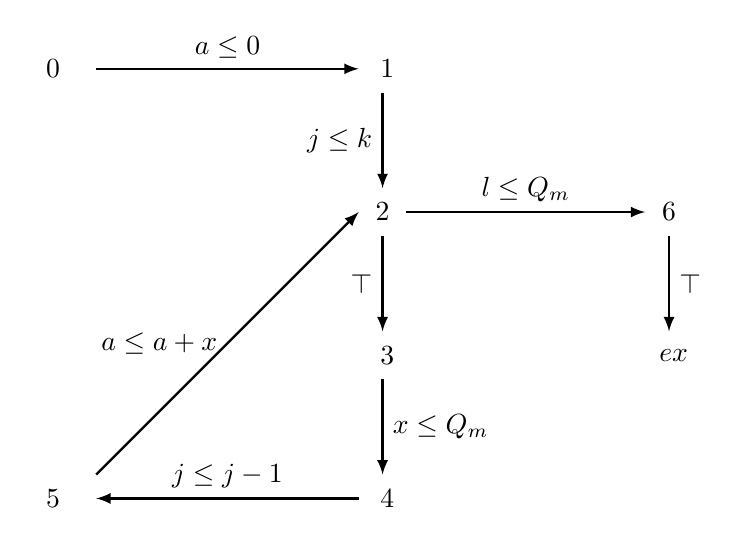
\begin{tikzpicture}[scale=\textwidth/20cm,samples=200]
  \draw[] (-7, 10) circle (0pt) node{{ $0$}};
  \draw[] (0, 10) circle (0pt) node{{ $1$}};
  \draw[] (0, 7) circle (0pt) node{\textbf{$2$}};
  \draw[] (0, 4) circle (0pt) node{{ $3$}};
  \draw[] (0, 1) circle (0pt) node{{ $4$}};
  \draw[] (-7, 1) circle (0pt) node{{ $5$}};
  % Counter Variables
  \draw[] (6, 7) circle (0pt) node {\textbf{$6$}};
  \draw[] (6, 4) circle (0pt) node {{ $ex$}};
  %
  % Control Flow Edges:
  \draw[ thick, -latex] (-6, 10)  -- node [above] {$a \leq 0$}(-0.5, 10);
  \draw[ thick, -latex] (0, 9.5)  -- node [left] {$j \leq k$} (0, 7.5) ;
  \draw[ thick, -latex] (0, 6.5)  -- node [left] {$\top$}  (0, 4.5);
  \draw[ thick, -latex] (0, 3.5)  -- node [right] {$x \leq Q_m$} (0, 1.5) ;
  \draw[ thick, -latex] (-0.5, 1)  -- node [above] {$j \leq j - 1$} (-6, 1) ;
  \draw[ thick, -latex] (-6, 1.5)  -- node [left] {$a \leq a + x$} (-0.5, 7)  ;
  \draw[ thick, -latex] (0.5, 7)  -- node [above] {$l \leq Q_m$}  (5.5, 7);
  \draw[ thick, -latex] (6, 6.5)  -- node [right] {$\top$} (6, 4.5) ;
  \end{tikzpicture}
  \caption{}
    \end{centering}
    \end{subfigure}
    \begin{subfigure}{.45\textwidth}
      \begin{centering}
    %   \todo{abstract-cfg for two round}
    \begin{tikzpicture}[scale=\textwidth/20cm,samples=200]
    \draw[] (-10, 10) circle (0pt) node{{ $0: 1$}};
    \draw[] (0, 10) circle (0pt) node{{ $1: 1$}};
    \draw[] (0, 7) circle (0pt) node{\textbf{$2: k$}};
    \draw[] (0, 4) circle (0pt) node{{ $3: k$}};
    \draw[] (0, 1) circle (0pt) node{{ $4: k$}};
    \draw[] (-10, 1) circle (0pt) node{{ $5: k$}};
    % Counter Variables
    \draw[] (6, 7) circle (0pt) node {\textbf{$6: 1$}};
    \draw[] (6, 4) circle (0pt) node {{ $ex: 1$}};
    %
    % Control Flow Edges:
  \draw[ thick, -latex] (-8, 10)  -- node [above] {$a \leq 0$}(-1.5, 10);
  \draw[ thick, -latex] (0, 9.5)  -- node [left] {$j \leq k$} (0, 7.5) ;
  \draw[ thick, -latex] (0, 6.5)  -- node [left] {$\top$}  (0, 4.5);
  \draw[ thick, -latex] (0, 3.5)  -- node [right] {$x \leq Q_m$} (0, 1.5) ;
  \draw[ thick, -latex] (-1.5, 1)  -- node [above] {$j \leq j - 1$} (-8, 1) ;
  \draw[ thick, -latex] (-8, 1.5)  -- node [left] {$a \leq a + x$} (-1.5, 7)  ;
  \draw[ thick, -latex] (1.5, 7)  -- node [above] {$l \leq Q_m$}  (4.5, 7);
  \draw[ thick, -latex] (6, 6.5)  -- node [right] {$\top$} (6, 4.5) ;
    \end{tikzpicture}
    \caption{}
      \end{centering}
      \end{subfigure}
    \caption{(a) The same $\kw{towRounds(k)}$ program as Figure~\ref{fig:twoRounds_example}
    (b) The abstract control flow graph for $\kw{towRounds(k)}$  (c) The abstract control flow graph with the reachability bound for $\kw{towRounds(k)}$.}
    \vspace{-0.5cm}
    \label{fig:abscfg_tworound}
  \end{figure}
\end{example}
% \section{Related Work}
% \label{sec:static-relatedwork}


\paragraph{{Static Analysis for Adaptivity Outline}}

In order to give a sound approximating this quantity, I design a static program analysis framework through three steps analysis
similar to the execution-based analysis in Chapter~\ref{sec:adapt-exe}.
% In order to give a sound approximating this quantity, I design a static program analysis framework through three steps analysis
% similar to the execution-based analysis in Section~\ref{sec:dynamic}.
% In this static program analysis, the program will be analysed in the same 3 aspects as the execution-based analysis 
%    while through static program analysis techniques, and a sound estimated result will be given in each aspect.
%    \\
% 	a. The data dependency relation analysis through the static data flow analysis technique.
%    \\
% 	b. The dependency quantity analysis through the static program reachability bound analysis techniques.
%    \\
% 	c. Combining the two analysis result above, I build a program-based dependency graph for approximating
%     the execution-based dependency graph. Then, I design an algorithm computing the adaptivity upper bound soundly 
%    and accurately on the program-based dependency graph.
\begin{itemize}
   \item In Section~\ref{sec:static-dep}
   The data \emph{dependency relation} analysis through the static data flow analysis technique.
   \item Still in Section~\ref{sec:static-quantity}, the \emph{dependency quantity} analysis through the static program reachability bound analysis techniques.
   \item The static analysis for adaptivity is presented in Section~\ref{sec:static-adapt}.
   % the program adaptivity estimation, 
   In this analysis, I construct a program-based dependence graph for approximating the execution-based graph in Section~\ref{sec:dynamic-adapt}.
   Then, based on this graph, I design an algorithm
   %  based on the results estimated above, 
   computing the adaptivity upper bound soundly 
   and accurately.
   \end{itemize}